\documentclass[tikz,border=2pt]{standalone}
\usepackage{amsmath,amssymb}
\usepackage{tikz}
\usetikzlibrary{arrows.meta}

\begin{document}
% The integers are equally spaced points on the number line, extending without end in both
% directions; the natural numbers are the ones from 0 to the right.
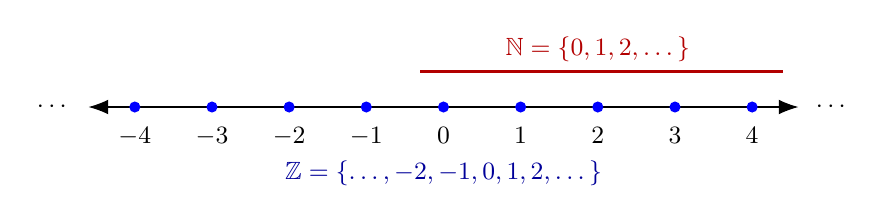
\begin{tikzpicture}[x=0.98cm]
	\draw[{Latex[length=2.5mm]}-{Latex[length=2.5mm]}] (-4.6,0) -- (4.6,0);
	\foreach \x in {-4,...,4} {\fill[blue] (\x,0) circle (2pt); \node[below=4pt, font=\small] at (\x,0) {$\x$};}
	\node[left, font=\small] at (-4.7,0) {$\cdots$};
	\node[right, font=\small] at (4.7,0) {$\cdots$};
	\draw[red!70!black, thick] (-0.3,0.45) -- (4.4,0.45);
	\node[red!70!black, above, font=\small] at (2,0.45) {$\mathbb{N}=\{0,1,2,\dots\}$};
	\node[blue!60!black, below=16pt, font=\small] at (0,0) {$\mathbb{Z}=\{\dots,-2,-1,0,1,2,\dots\}$};
\end{tikzpicture}
\end{document}
